\documentclass[border=15pt]{standalone}
\usepackage{amsmath, amssymb}
\usepackage{tikz}
\usetikzlibrary{arrows.meta}

\definecolor{block0}{HTML}{E53935}
\definecolor{block1}{HTML}{1E88E5}
\definecolor{block2}{HTML}{43A047}
\definecolor{block3}{HTML}{FB8C00}
\definecolor{block4}{HTML}{8E24AA}
\definecolor{block5}{HTML}{00ACC1}
\definecolor{block6}{HTML}{F4511E}
\definecolor{block7}{HTML}{3949AB}

\begin{document}
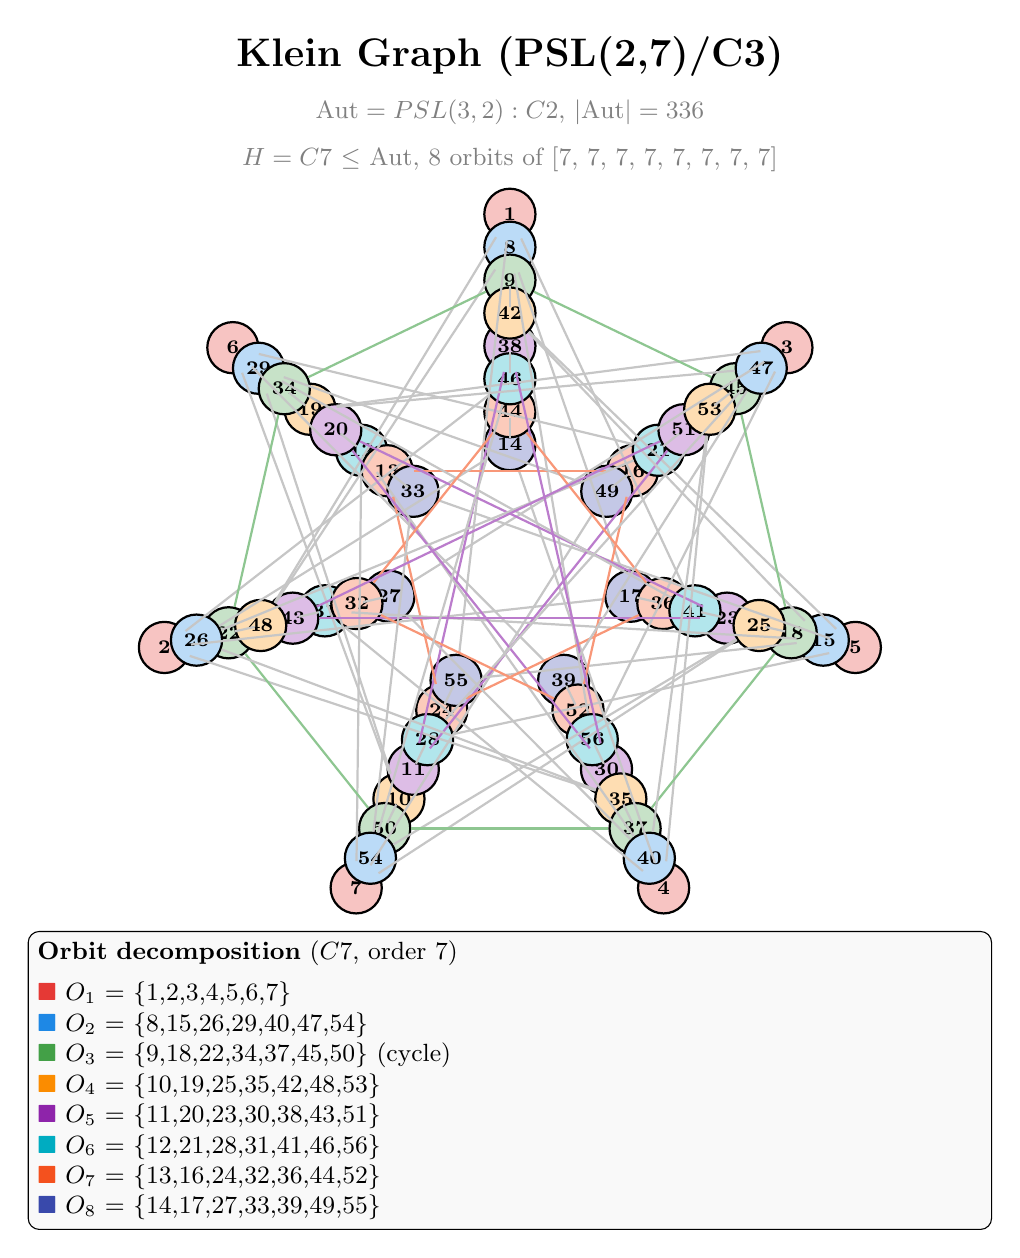
\begin{tikzpicture}[
  vertex/.style={circle, draw, thick, minimum size=6.5mm, inner sep=0pt,
                 font=\scriptsize\bfseries},
  edge/.style={thick, gray!45},
  title/.style={font=\Large\bfseries},
  subtitle/.style={font=\small, text=gray},
]

\node[title] at (0, 6.5) {Klein Graph (PSL(2,7)/C3)};
\node[subtitle] at (0, 5.8) {$\mathrm{Aut} = PSL(3,2) : C2$, $|\mathrm{Aut}| = 336$};
\node[subtitle] at (0, 5.2) {$H = C7$ $\leq$ $\mathrm{Aut}$, 8 orbits of [7, 7, 7, 7, 7, 7, 7, 7]};

\node[vertex, fill=block0!30] (v1) at (0.000, 4.500) {1};
\node[vertex, fill=block0!30] (v2) at (-4.387, -1.001) {2};
\node[vertex, fill=block0!30] (v3) at (3.518, 2.806) {3};
\node[vertex, fill=block0!30] (v4) at (1.952, -4.054) {4};
\node[vertex, fill=block0!30] (v5) at (4.387, -1.001) {5};
\node[vertex, fill=block0!30] (v6) at (-3.518, 2.806) {6};
\node[vertex, fill=block0!30] (v7) at (-1.952, -4.054) {7};
\node[vertex, fill=block1!30] (v8) at (0.000, 4.082) {8};
\node[vertex, fill=block2!30] (v9) at (0.000, 3.664) {9};
\node[vertex, fill=block3!30] (v10) at (-1.409, -2.925) {10};
\node[vertex, fill=block4!30] (v11) at (-1.227, -2.548) {11};
\node[vertex, fill=block5!30] (v12) at (-1.885, 1.503) {12};
\node[vertex, fill=block6!30] (v13) at (-1.558, 1.243) {13};
\node[vertex, fill=block7!30] (v14) at (0.000, 1.575) {14};
\node[vertex, fill=block1!30] (v15) at (3.980, -0.908) {15};
\node[vertex, fill=block6!30] (v16) at (1.558, 1.243) {16};
\node[vertex, fill=block7!30] (v17) at (1.536, -0.350) {17};
\node[vertex, fill=block2!30] (v18) at (3.572, -0.815) {18};
\node[vertex, fill=block3!30] (v19) at (-2.538, 2.024) {19};
\node[vertex, fill=block4!30] (v20) at (-2.211, 1.764) {20};
\node[vertex, fill=block5!30] (v21) at (1.885, 1.503) {21};
\node[vertex, fill=block2!30] (v22) at (-3.572, -0.815) {22};
\node[vertex, fill=block4!30] (v23) at (2.758, -0.629) {23};
\node[vertex, fill=block6!30] (v24) at (-0.865, -1.796) {24};
\node[vertex, fill=block3!30] (v25) at (3.165, -0.722) {25};
\node[vertex, fill=block1!30] (v26) at (-3.980, -0.908) {26};
\node[vertex, fill=block7!30] (v27) at (-1.536, -0.350) {27};
\node[vertex, fill=block5!30] (v28) at (-1.046, -2.172) {28};
\node[vertex, fill=block1!30] (v29) at (-3.192, 2.545) {29};
\node[vertex, fill=block4!30] (v30) at (1.227, -2.548) {30};
\node[vertex, fill=block5!30] (v31) at (-2.350, -0.536) {31};
\node[vertex, fill=block6!30] (v32) at (-1.943, -0.443) {32};
\node[vertex, fill=block7!30] (v33) at (-1.231, 0.982) {33};
\node[vertex, fill=block2!30] (v34) at (-2.865, 2.285) {34};
\node[vertex, fill=block3!30] (v35) at (1.409, -2.925) {35};
\node[vertex, fill=block6!30] (v36) at (1.943, -0.443) {36};
\node[vertex, fill=block2!30] (v37) at (1.590, -3.301) {37};
\node[vertex, fill=block4!30] (v38) at (0.000, 2.829) {38};
\node[vertex, fill=block7!30] (v39) at (0.683, -1.419) {39};
\node[vertex, fill=block1!30] (v40) at (1.771, -3.678) {40};
\node[vertex, fill=block5!30] (v41) at (2.350, -0.536) {41};
\node[vertex, fill=block3!30] (v42) at (0.000, 3.246) {42};
\node[vertex, fill=block4!30] (v43) at (-2.758, -0.629) {43};
\node[vertex, fill=block6!30] (v44) at (0.000, 1.993) {44};
\node[vertex, fill=block2!30] (v45) at (2.865, 2.285) {45};
\node[vertex, fill=block5!30] (v46) at (0.000, 2.411) {46};
\node[vertex, fill=block1!30] (v47) at (3.192, 2.545) {47};
\node[vertex, fill=block3!30] (v48) at (-3.165, -0.722) {48};
\node[vertex, fill=block7!30] (v49) at (1.231, 0.982) {49};
\node[vertex, fill=block2!30] (v50) at (-1.590, -3.301) {50};
\node[vertex, fill=block4!30] (v51) at (2.211, 1.764) {51};
\node[vertex, fill=block6!30] (v52) at (0.865, -1.796) {52};
\node[vertex, fill=block3!30] (v53) at (2.538, 2.024) {53};
\node[vertex, fill=block1!30] (v54) at (-1.771, -3.678) {54};
\node[vertex, fill=block7!30] (v55) at (-0.683, -1.419) {55};
\node[vertex, fill=block5!30] (v56) at (1.046, -2.172) {56};

\draw[edge] (v1) -- (v41);
\draw[edge] (v1) -- (v48);
\draw[edge] (v1) -- (v55);
\draw[edge] (v2) -- (v17);
\draw[edge] (v2) -- (v35);
\draw[edge] (v2) -- (v46);
\draw[edge] (v3) -- (v19);
\draw[edge] (v3) -- (v27);
\draw[edge] (v3) -- (v56);
\draw[edge] (v4) -- (v14);
\draw[edge] (v4) -- (v31);
\draw[edge] (v4) -- (v53);
\draw[edge] (v5) -- (v28);
\draw[edge] (v5) -- (v33);
\draw[edge] (v5) -- (v42);
\draw[edge] (v6) -- (v10);
\draw[edge] (v6) -- (v21);
\draw[edge] (v6) -- (v39);
\draw[edge] (v7) -- (v12);
\draw[edge] (v7) -- (v25);
\draw[edge] (v7) -- (v49);
\draw[edge] (v8) -- (v17);
\draw[edge] (v8) -- (v48);
\draw[edge] (v8) -- (v56);
\draw[thick, block2!60] (v9) -- (v34);
\draw[edge] (v9) -- (v42);
\draw[thick, block2!60] (v9) -- (v45);
\draw[edge] (v10) -- (v29);
\draw[edge] (v10) -- (v50);
\draw[edge] (v11) -- (v28);
\draw[thick, block4!60] (v11) -- (v38);
\draw[thick, block4!60] (v11) -- (v51);
\draw[edge] (v12) -- (v20);
\draw[edge] (v12) -- (v40);
\draw[thick, block6!60] (v13) -- (v16);
\draw[thick, block6!60] (v13) -- (v24);
\draw[edge] (v13) -- (v33);
\draw[edge] (v14) -- (v26);
\draw[edge] (v14) -- (v44);
\draw[edge] (v15) -- (v31);
\draw[edge] (v15) -- (v42);
\draw[edge] (v15) -- (v55);
\draw[edge] (v16) -- (v49);
\draw[thick, block6!60] (v16) -- (v52);
\draw[edge] (v17) -- (v36);
\draw[edge] (v18) -- (v25);
\draw[thick, block2!60] (v18) -- (v37);
\draw[thick, block2!60] (v18) -- (v45);
\draw[edge] (v19) -- (v34);
\draw[edge] (v19) -- (v47);
\draw[thick, block4!60] (v20) -- (v23);
\draw[thick, block4!60] (v20) -- (v30);
\draw[edge] (v21) -- (v26);
\draw[edge] (v21) -- (v51);
\draw[thick, block2!60] (v22) -- (v34);
\draw[edge] (v22) -- (v48);
\draw[thick, block2!60] (v22) -- (v50);
\draw[edge] (v23) -- (v41);
\draw[thick, block4!60] (v23) -- (v43);
\draw[thick, block6!60] (v24) -- (v36);
\draw[edge] (v24) -- (v55);
\draw[edge] (v25) -- (v54);
\draw[edge] (v26) -- (v35);
\draw[edge] (v27) -- (v32);
\draw[edge] (v27) -- (v40);
\draw[edge] (v28) -- (v47);
\draw[edge] (v29) -- (v41);
\draw[edge] (v29) -- (v49);
\draw[thick, block4!60] (v30) -- (v38);
\draw[edge] (v30) -- (v56);
\draw[edge] (v31) -- (v43);
\draw[thick, block6!60] (v32) -- (v44);
\draw[thick, block6!60] (v32) -- (v52);
\draw[edge] (v33) -- (v54);
\draw[edge] (v35) -- (v37);
\draw[thick, block6!60] (v36) -- (v44);
\draw[thick, block2!60] (v37) -- (v50);
\draw[edge] (v38) -- (v46);
\draw[edge] (v39) -- (v47);
\draw[edge] (v39) -- (v52);
\draw[edge] (v40) -- (v53);
\draw[thick, block4!60] (v43) -- (v51);
\draw[edge] (v45) -- (v53);
\draw[edge] (v46) -- (v54);

\node[draw, rounded corners, fill=gray!5, text width=12cm, align=left, font=\small]
  at (0, -6.5) {
  \textbf{Orbit decomposition} ($C7$, order 7) \\[4pt]
  \textcolor{block0}{$\blacksquare$} $O_{1}$ = \{1,2,3,4,5,6,7\} \\
  \textcolor{block1}{$\blacksquare$} $O_{2}$ = \{8,15,26,29,40,47,54\} \\
  \textcolor{block2}{$\blacksquare$} $O_{3}$ = \{9,18,22,34,37,45,50\} (cycle) \\
  \textcolor{block3}{$\blacksquare$} $O_{4}$ = \{10,19,25,35,42,48,53\} \\
  \textcolor{block4}{$\blacksquare$} $O_{5}$ = \{11,20,23,30,38,43,51\} \\
  \textcolor{block5}{$\blacksquare$} $O_{6}$ = \{12,21,28,31,41,46,56\} \\
  \textcolor{block6}{$\blacksquare$} $O_{7}$ = \{13,16,24,32,36,44,52\} \\
  \textcolor{block7}{$\blacksquare$} $O_{8}$ = \{14,17,27,33,39,49,55\}
};

\end{tikzpicture}
\end{document}